\chapter{Primeri medplatformnega razvoja aplikacij}

Obravnavali smo štiri različne metode PlayN, Unity, WebGL in C++. Za vsako smo razvili aplikacijo in izpostavili prednosti in slabosti metode. Vsi primeri so dostopni na spletnem naslovu \texttt{http://diploma.pecar.me/}.

\section{Učenje tujih jezikov}

\subsection{Opis problema}

Prvi primer je preprosta grafična aplikacija, ki uporabnikom olajša učenje tujih jezikov. Deluje na preprostem principu pomnjenja besed. Igralcu se na zaslonu pokaže beseda v domačem jeziku in tri besede v jeziku, ki se ga uporabnik skuša naučiti. Dve besedi sta naključno izbrani, tretja pa je pravilni odgovor. Vrstni red besed je naključen.

V primeru pravilnega odgovora se uporabniku pokaže naslednja beseda in trije novi odgovori. Tako uporabnik nadaljuje z učenjem. Če uporabnik izbere napačni odgovor, se na zaslonu pojavi pravilni prevod besede. Na ta način ima uporabnik možnost naučiti se novo besedo. Ko si uporabnik ogleda pravilni odgovor, se igra ponovno začne.

Primer delovanja aplikacije je na sliki \ref{german}, kjer je viden glavni zaslon aplikacije s tremi možnimi odgovori.

\begin{figure}
\begin{center}
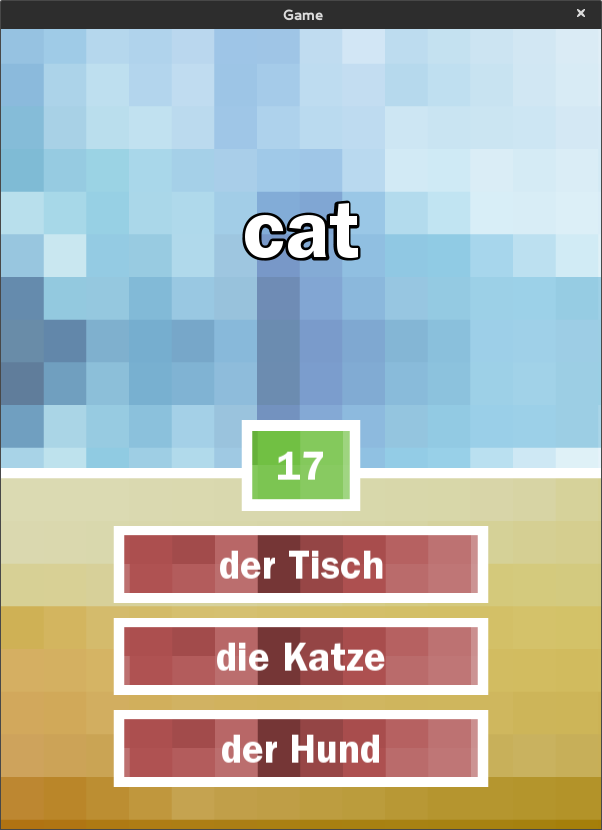
\includegraphics[width=5.5cm]{pic/defg-german.png}
\end{center}
\caption{Primer delovanja nemške verzije na namiznem računalniku}
\label{german}
\end{figure} 

Ena izmed glavnih zahtev igre je izpis različnih pisav in posebnih znakov. Poleg prikazane verzije nemščina - angleščina, je bila aplikacija razvita tudi z idejo učenja jezikov, ki ne uporabljajo latinice. Slika \ref{korean} prikazuje primer učenja korejščine. 

\begin{figure}
\begin{center}
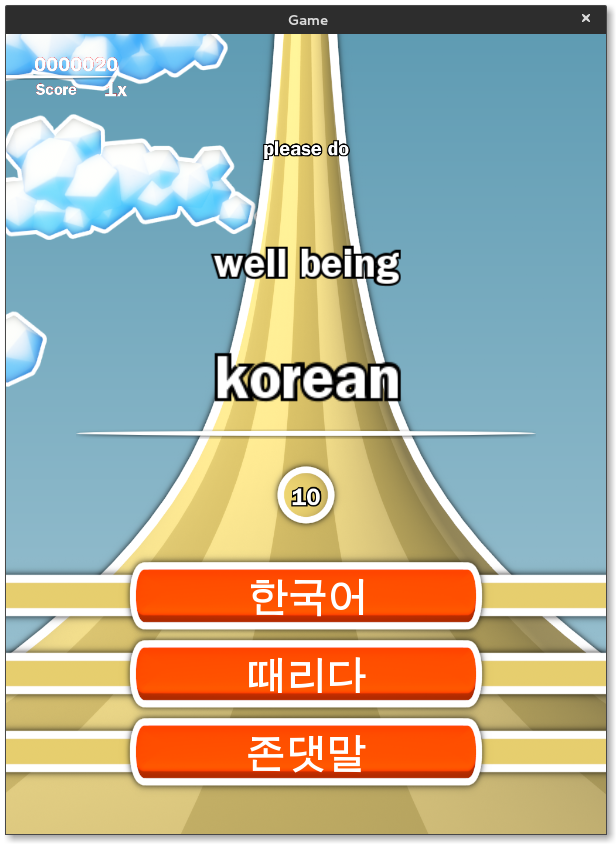
\includegraphics[width=5.5cm]{pic/defg-korean.png}
\end{center}
\caption{Primer delovanja korejske verzije na mobilni napravi}
\label{korean}
\end{figure} 

\subsection{Uporabljena metoda}

Izmed vseh obravnavanih metod se nam je zdela najbolj primerna metoda PlayN. Razlogi za izbiro metode so naslednji:

\begin{itemize}
\item PlayN je odprtokoden projekt. V primeru težav lahko pogledamo v izvorno kodo projekta in po potrebi težave odpravimo sami.
\item Licenca, ki jo PlayN uporablja, ni omejujoča in v primerjavi z nekaterimi plačljivimi metodami ne zahteva nobenega plačila pred uporabo. To velja tudi, če bi aplikacijo uporabili za komercialne namene.
\item PlayN je še vedno v aktivnem razvoju, razvijalci pa so odzivni na listi za elektronsko pošto.
\item PlayN omogoča preprosto podporo dodajanju lastnih pisav, kar je ključ-nega pomena za podporo jezikom kot je korejščina.
\item Število platform, ki jih PlayN podpira, zadošča potrebam aplikacije.
\item PlayN omogoča uporabo vročega izmenjevanja kode, kar zelo pohitri razvoj aplikacije.
\item Poleg samega ogrodja PlayN je na voljo tudi precej vtičnikov, ki so jih razvili uporabniki. Tak primer je vtičnik Tripleplay, ki je v aplikaciji uporabljen za prikaz menijev.
\item Dokumentacija je dobro urejena.
\end{itemize}

\subsection{Opis metode}

Projekt z uporabo pogona PlayN sestavlja več imenikov. Glavni imenik se imenuje \texttt{core} in vsebuje logiko celotne aplikacije. Izvorna koda, ki se nahaja v tem imeniku, definira kaj se bo na zaslonu prikazalo ter kako se aplikacija odziva na vnose uporabnikov. 



Imenik \texttt{assets} služi kot imenik vseh sredstev, ki jih aplikacija potrebuje za delovanje. V imeniku se nahaja vsa grafika, ki je v uporabi v aplikaciji, in vse zvočne datoteke.

Ostali imeniki so namenjeni posameznim platformam. Imenik \texttt{java} vsebuje preprost program, ki odpre okno in nastavi grafično okolje. Ko je okno pripravljeno, pokliče glavno metodo imenika \texttt{core} in aplikacija se začne izvajati. Podobno delujeta tudi imenika \texttt{android} in \texttt{ios}, vsak za svojo platformo. Oba definirata vse potrebno za zagon na sistemih Android in iOS in nato pokličeta metodo iz imenika \texttt{core}.

Aplikacija mora biti sposobna izrisovati velik nabor različnih abeced. To dejstvo je močno vplivalo na izbor metode. PlayN podpira tako 3D kot 2D vmesnik za izrisovanje, vendar smo se zaradi kompleksnosti izrisovanja različnih pisav s 3D vmesnikom odločili za uporabo 2D vmesnika. Naložitev lastnih pisav v projekt je zelo preprosta. Datoteko dodamo v imenik \texttt{assets}, iz programske kode pa pisavo registriramo s pomočjo metode \texttt{public void registerFont(String name, String path)} in nato uporabimo z uporabo metode \texttt{Font createFont(String name, Font.Style style, float size)}. Pisava, ki jo vrne zadnja metoda, je tako na voljo za uporabo.

Pomembna zahteva aplikacije je bila tudi delovanje na mobilnih platformah iOS in Android. Tudi tu nam je ogrodje PlayN olajšalo delo, saj postavitev delovnega okolja ni bilo težavno. Proces izvoza aplikacije na različne platforme poteka z uporabo orodij Ant ali Maven. Maven je orodje za upravljanje s projekti, ki skrbi za grajenje projektov in njihovo dokumentacijo \cite{mvn}. PlayN ima že predpripravljene nastavitve za Maven. Za grajenje Android aplikacije moramo izvesti samo preprost ukaz: \texttt{mvn install -Pandroid}. 

Namizna aplikacija ima obliko izvedljive \texttt{jar} datoteke, ki jo moramo pripraviti sami. PlayN nima predpripravljenih navodil za izgradnjo \texttt{jar} datoteke, vendar lahko to preprosto storimo znotraj razvijalskega orodja Eclipse. Pazljivi moramo biti le, da poleg \texttt{jar} datoteke dodamo tudi domorodne knjižnice pritikline LWJGL. LWJGL \cite{lwjgl} omogoča dostop do vmesnikov za OpenGL, OpenCL in OpenAL na operacijskih sistemih FreeBSD, Linux, Mac OSX, Solaris in Windows.

Poleg verzije za mobilne naprave in namizne računalnike lahko izvozimo tudi verzijo za spletne brskalnike. Za grajenje spletne aplikacije uporabimo orodje Maven z ukazom \texttt{mvn -Phtml integration-test}. Ukaz nam zažene Jetty spletni strežnik, na katerem je dostopna naša aplikacija. Orodje Maven ima tudi dodatek, ki nam aplikacijo pošlje na Googlov AppEngine. Naša verzija za spletne brskalnike deluje zadovoljivo tudi na mobilnih napravah.

\subsection{Prednosti izbora metode}

Izbrana metoda nam je pomagala izpolniti vse zastavljene cilje. Brez truda smo aplikacijo razvijali na namiznem računalniku in po potrebi preizkusili delovanje na Android napravi. Vmesnik API je razumljiv. Krivulja učenja ni bila strma. 

\subsection{Slabosti izbora metode}

Težave smo imeli pri preizkušanju verzije za iOS naprave. Kljub izčrpni dokumentaciji smo naleteli na probleme s konflikti med pritiklinami ogrodja PlayN. Z nekaj raziskovanja nam je vse probleme uspelo odpraviti. 

Težave je povzročil tudi prehod iz verzije 1.6 na 1.7, ki se je zgodil med razvojem aplikacije. Nova verzija je malce spremenila način dela s sredstvi in potrebnih je bilo nekaj ročnih popravkov strukture projekta, da sta Android in iOS verziji ponovno delovali.

\section{Štiri v vrsto}

Druga testna aplikacija je preprosta igra štiri v vrsto, postavljena v treh dimenzijah. Ideja aplikacije je skozi preprosto igro izboljšati uporabnikovo orientacijo v 3D prostoru. Za razliko od standardne igre štiri v vrsto, kjer so zmagovalne kombinacije omejene v vodoravni, navpični in horizontalni smeri, imamo v 3D verziji veliko več možnosti. Poleg osnovnih smeri lahko zmagovalno kombinacijo zgradimo tudi v globino, kar odpre obilico novih kombinacij.

Igra se začne, ko prvi igralec z dotikom na valj postavi prvo kocko. Drugi igralec nato na podoben način postavi svojo prvo kocko, ki pa se barvno loči od kocke prvega igralca. Igralca se na tak način izmenjujeta, dokler eden izmed njiju ne uspe postaviti štirih kock v vrsto. Takrat se zmagovalne kocke odebelijo in igra se konča.

Za lažjo orientacijo v prostoru igre je igralno površino možno obračati. Obračanje poteka tako, da s klikom na miško ali z dotikom na dotik občutljivi zaslon potegnemo po okolici igralne površine. Kamera se pomakne okoli središča glede na dolžino potega. Razdalja med kamero in središčem se ne spreminja. Prav tako se ne spremeni smer kamere, ki ves čas gleda proti središču igralne površine.

\subsection{Uporabljena metoda}

Za razvoj smo se odločili za orodje Unity. Unity za razliko od ostalih metod, ki smo jih preučevali, vključuje lastno integrirano razvojno okolje. Integrirano razvojno okolje prikazuje slika \ref{mineditor}. Omogoča nam postavljanje objektov v sceno, postavitev kamere, določitev luči in še množico drugih stvari, vse preko grafičnega vmesnika. Za postavitev objektov v 3D prostor imamo na voljo okno z ortografsko ali perspektivno projekcijo. Na preprost način si sceno lahko ogledamo z različnih zornih kotov.


\begin{figure}
\begin{center}
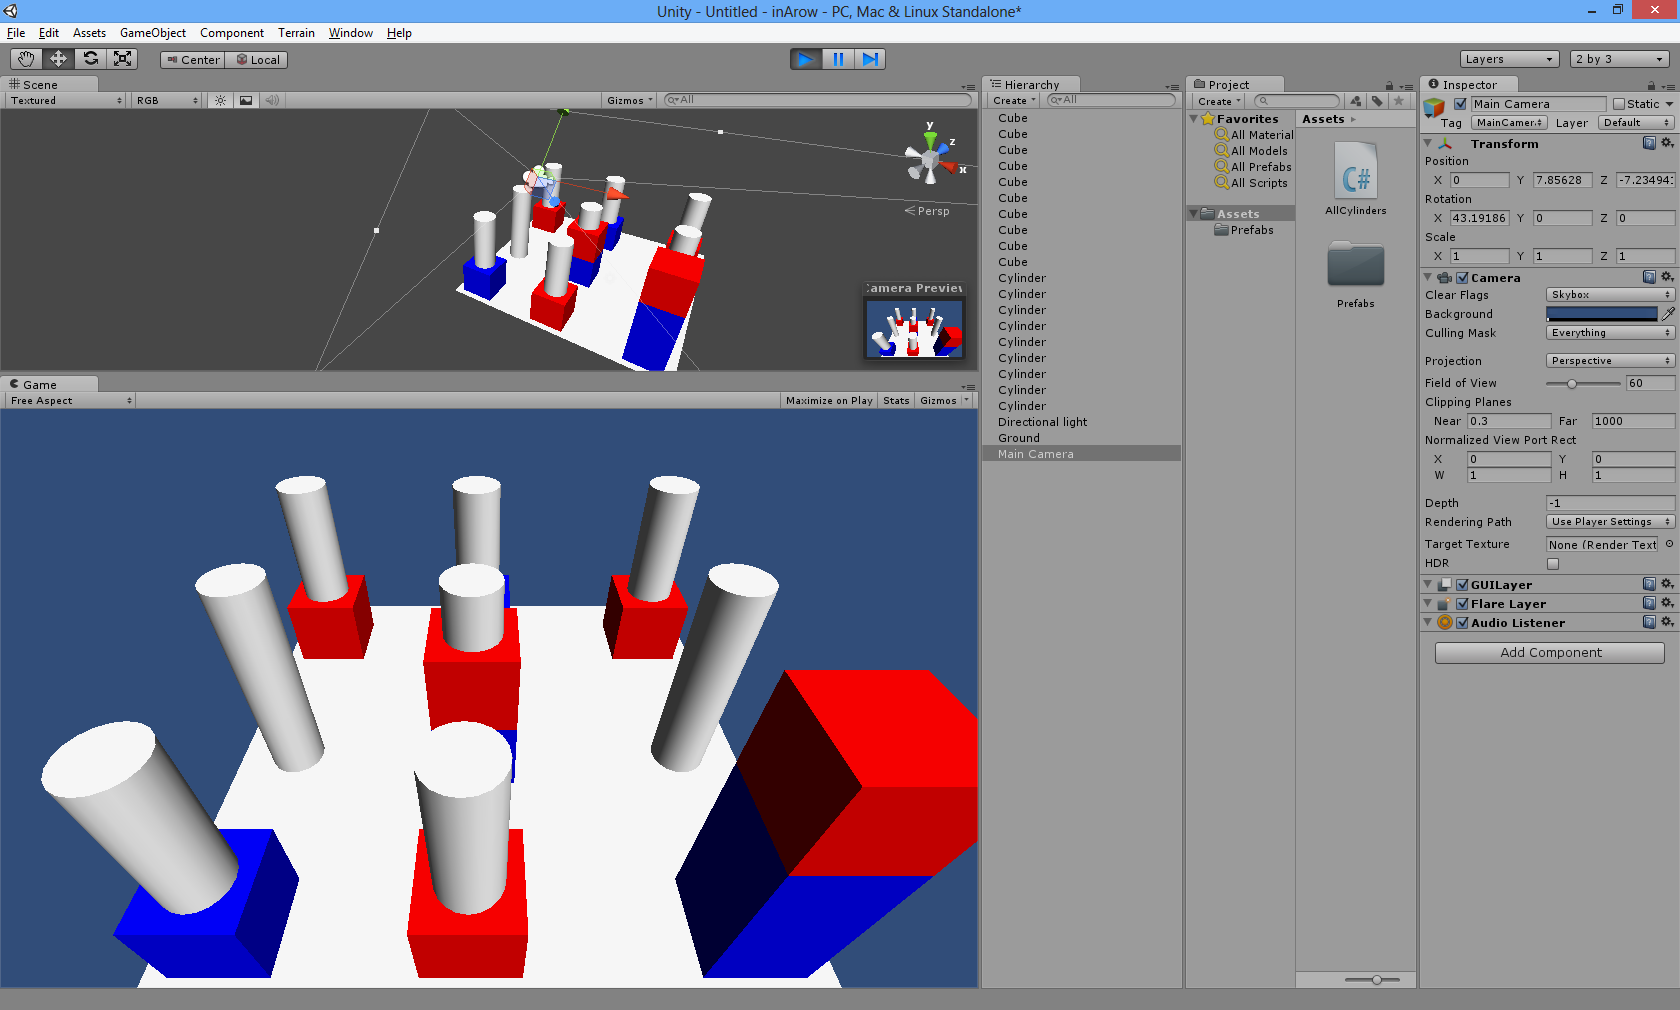
\includegraphics[width=12cm]{pic/min-editor.png}
\end{center}
\caption{Razvoj grafično intenzivne aplikacije v okolju Unity.}
\label{mineditor}
\end{figure} 

\begin{figure}
\begin{center}
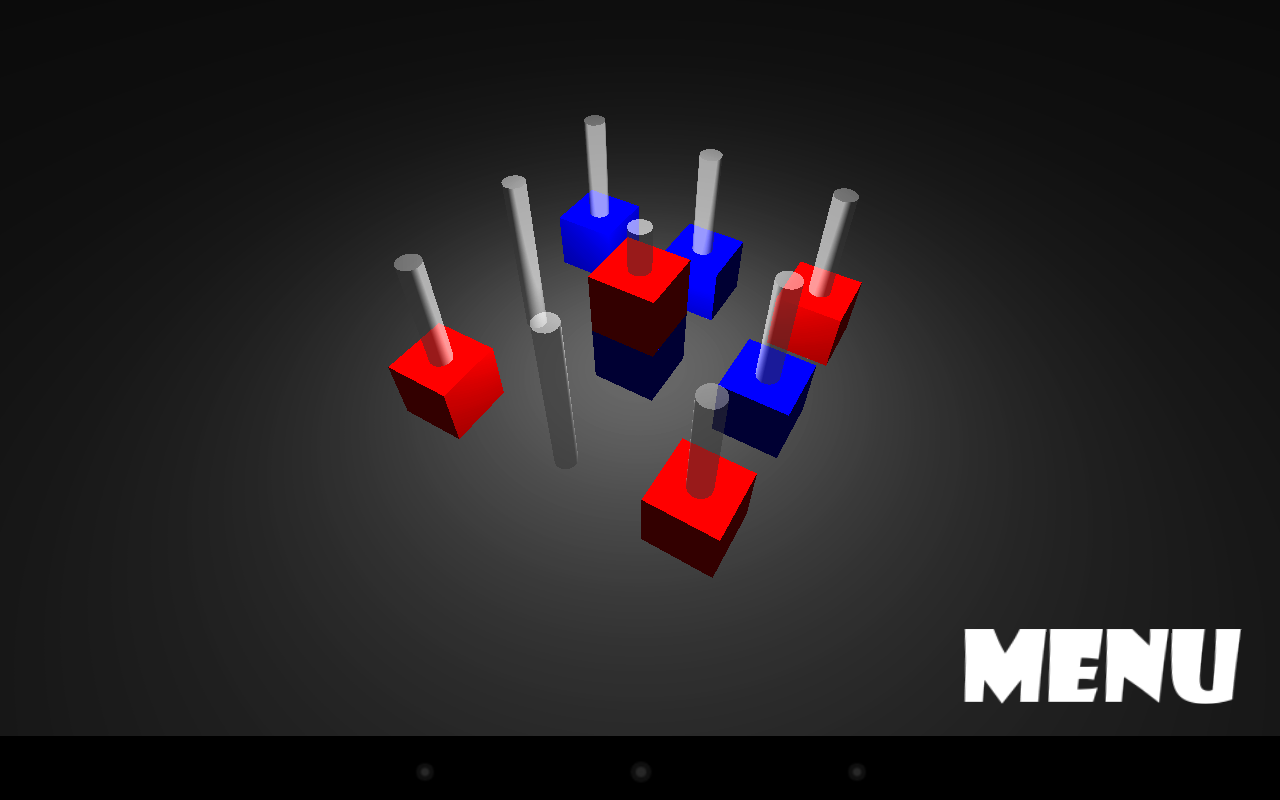
\includegraphics[width=10cm]{pic/min-play.png}
\end{center}
\caption{Končana Unity aplikacija izvožena na mobilno platformo.}
\label{minplay}
\end{figure} 

S pomočjo integriranega razvojnega okolja lahko določimo tudi različne lastnosti posameznih objektov. Te lastnosti so določitev materiala, različni sprožilci za dogodke in tip senc, ki jih objekt ustvarja. Za logiko, obnašanje in odziv na uporabniški vhod lahko vsakemu objektu dodelimo tudi skriptno datoteko. V skriptni datoteki v enem od podprtih programskih jezikih (C\#, JavaScript, Boo) določimo, kako se bo objekt odzival na različne dejavnike in kako se bo obnašal v času, ko je viden na zaslonu.

Aplikacija ima preprosto zasnovo. Ko se igra zažene, se ustvarijo prazni valji, na katere se nastavi dogodek \texttt{addBlock}, ki se sproži ob dotiku na valj. Unity okolje avtomatično prevede koordinate zaslona v koordinate prostora in pravilno določi valj, ki smo se ga dotaknili. Prav tako orodje Unity abstrahira različne vrste vhoda, bodisi klik z miško ali dotik na dotik občutljivem zaslonu.

Dogodek \texttt{addBlock} na izbrani valj položi novo barvasto kocko - rdečo ali modro, odvisno, kateri igralec je na voljo. Nova kocka se tudi doda na seznam, ki interno predstavlja stanje igralne plošče. Algoritem nato preveri novo stanje seznama. Če se je z zadnjo potezo pojavila zmagovalna kombinacija, se igra konča.

Ko se igra konča, se pojavi besedilo, ki sporoči zmagovalca in ponudi ponovno igranje. V bolj pogostem primeru, ko poteza ne zaključi igre, se samo zamenja aktivni igralec in igra se nadaljuje. 

Izvoz na različne platforme poteka preko posebnega dialoga za grajenje aplikacije (\texttt{File - Build Settings...}). V dialogu določimo ciljno platformo in nastavitve. S klikom na gumb \texttt{Build} se aplikacija prevede in zgradi za ciljno platformo. V primeru PC, Mac in Linux verzij kot rezultat grajenja dobimo binarno datoteko, ki je izvedljiva na teh platformah. V primeru iOS in Android aplikacij nam lahko Unity pripravi projekt, ki ga nato odpremo v orodjih Eclipse ali Xcode. Tako lahko aplikacijo podpišemo in pripravimo za objavo v trgovinah z mobilnimi aplikacijami. Slika \ref{minplay} prikazuje delovanje aplikacije na platformi Android.

\subsection{Prednosti metode}

Unity urejevalnik nam je omočil zelo hiter razvoj aplikacije, saj je bilo ustvarjanje osnovnih oblik in postavitev le-teh v prostor zelo preprosto. Tudi pisanje skriptnih datotek za obnašanje in logiko aplikacije ni bilo težavno.

\subsection{Slabosti metode}

Problem uporabe orodja Unity je učna krivulja. Za razliko od večine ostalih metod se moramo poleg vmesnika API naučiti tudi dela s priloženim urejevalnikom. Sicer je urejevalnik preprost za uporabo, vendar učenje vseh potrebnih operacij vzame precej časa.

Druga slabost metode je v zaprtost sistema. Če v času razvoja aplikacije naletimo na omejitev orodja, nimamo dostopa do izvorne kode, kjer bi to omejitev lahko odpravili. Orodje je sicer na voljo brezplačno, vendar moramo za uporabo naprednih funkcij kupiti licenco. Aplikacije razvite z brezplačno verzijo programa imajo na vseh platformah pred zagonom na zaslonu napis Unity. 

\section{Igra MIN}

Tretji primer je preprosta igra, ki uporablja ortografsko projekcijo. Cilj igre je s sivo kocko odstraniti rdeče kocke. Sivo kocko premika igralec, rdeče kocke pa so postavljene v obliki ugank. Premikanje sive kocke levo, desno, navzgor in navzdol je možno samo v naprej določenih perspektivah. 

V ptičji perspektivi, kjer vidimo pozicije vseh rdečih kock, premikanje sploh ni možno. V drugi perspektivi se lahko premikamo samo levo in desno, zaradi ortografske projekcije pa ne ločimo, katere kocke so višje ali nižje od nas. V tretji perspektivi se lahko premikamo navzgor in navzdol, ne vidimo pa več, katere kocke so levo in katere desno od nas. Zaradi omejenega gibanja si mora igralec v glavi ustvariti celotno sliko igralnega polja. Če se med spreminjanjem perspektive siva kocka dotakne črne črte, se igrana stopnja ponastavi. Slika \ref{minff} prikazuje delovanje končane aplikacije v mobilnem brskalniku.

Igra na prvi pogled deluje kot preprosta 2D aplikacija, vendar animirani prehodi med posameznimi perspektivami močno otežijo uporabo 2D platna. Iz tega razloga smo se odločili za uporabo 3D platna WebGL. %Animirani prehodi niso edini razlog zakaj se nismo odločili za bolje podprto 2D platno. Računanje pozicij posameznih kock v različnih perspektivah bi bilo težje izvedljivo, kot z uporabo WebGLa, kjer efekt dosežemo s preprostim prestavljanjem kamere.

\begin{figure}
\begin{center}
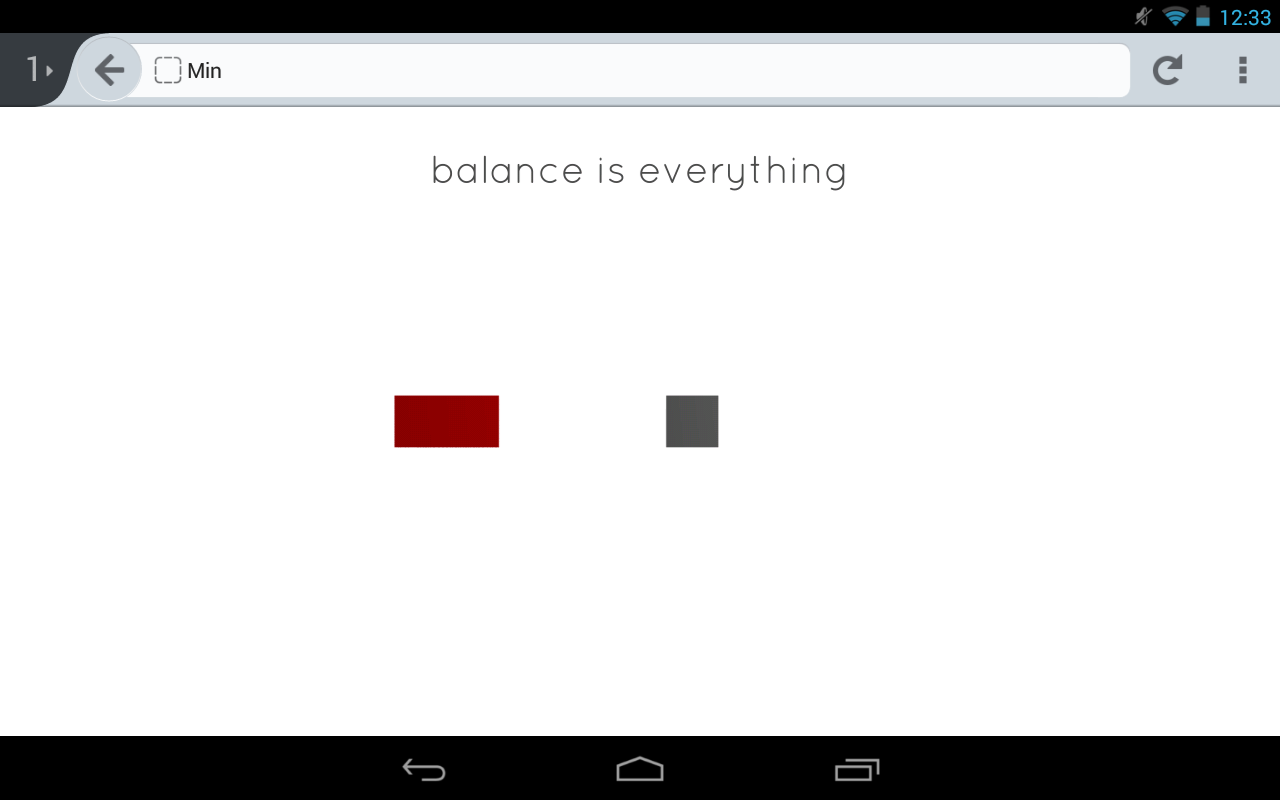
\includegraphics[width=12cm]{pic/min-ff.png}
\end{center}
\caption{Delovanje igre v mobilnem brskalniku Firefox.}
\label{minff}
\end{figure}

\subsection{Uporabljena metoda}

Za lažje delo z WebGLom smo uporabili knjižnico THREE.js, ki poenostavi delo s 3D objekti. Uporabili smo tudi knjižnico hammer.js, ki nam pomaga zaznavati geste na dotik občutljivem zaslonu.

\subsection*{THREE.js}

THREE.js je knjižnica za delo z WebGLom. Ponudi nam pester nabor uporabnih metod, ki močno poenostavijo izrisovanje modelov, določanje materialov, postavitev kamere in različnih luči v sceno. Knjižnica pripravi tudi potrebne senčilnike tako, da uporabniku ni potrebno pisati GLSL izvorne kode. Pisanje lastnih senčilnikov vseeno obstaja kot opcija.

Nastavitev ortografske kamere je v knjižnici THREE.js zelo preprosta. Potreben je samo klic posebne metode \texttt{THREE.OrthographicCamera(left, right, top, bottom, near, far)} s pravilnimi parametri. Kamero premikamo po prostoru na podoben način kot vse ostale objekte - z nastavljanjem parametra 3D vektorja \texttt{position}. 

V sceno smo dodali tudi dve točkovni luči. Prvo smo postavili na rob igralne plošče tako, da poudari stranice kock v različnih perspektivah. Druga luč pa se nahaja nad igralno površino, tako da so kocke od zgoraj navzdol dobro osvetljene. Dodajanje luči v sceno poteka v dveh korakih. Najprej ustvarimo objekt \texttt{var light =  new THREE.PointLight(0xFFF);}, ki ga nato dodamo v sceno \texttt{scene.add(light);}.

Na osebnih računalnikih premikamo kocko z uporabo smernih tipk, prehod med posameznimi perspektivami pa delamo s preslednico. Na mobilnih napravah nimamo na voljo fizične tipkovnice, navidezne pa zasedejo veliko prostora na zaslonu in tudi tipkanje je težavnejše. Zaradi tega na mobilnih napravah kocko uporabljamo s pomočjo gest. Za lažje delo z gestami smo uporabili knjižnico Hammer.js.

\subsection*{Hammer.js}

Hammer.js je JavaScript knjižnica za zaznavanje gest. Na podlagi standardnih dogodkov, ki jih brskalniki sprožijo ob dotiku zaslona, knjižnica ustvari nove, višje nivojske dogodke, ki se sprožijo ob posameznih gestah. Tako se lahko naročimo na te višje nivojske dogodke in smo obveščeni, ko uporabnik aplikacije izvede določeno gesto.

Višje nivojski dogodki so tipa poteg desno, poteg levo, dvoprstni poteg in tako dalje. 

Na podoben način se lahko naročimo tudi na druge vrste dogodkov, med katere spadajo potegi v vse možne smeri, daljši pritisk, kratek pritisk, uščip za povečavo in tako naprej.

Knjižnica omogoča tudi nastavitve posameznih gest, kot so dolžina pritiska potrebna za dogodek daljši pritisk, tako da lahko delovanje knjižnice prilagodimo našim specifičnim zahtevam. Za delovanje naše aplikacije to ni bilo potrebno.

\subsection{Prednosti izbora metode}

Izbrana metoda nam je omogočila hiter razvoj aplikacije. Aplikacijo smo razvijali na namiznem računalniku, kjer moderni brskalniki (Chrome, Firefox) podpirajo celo simuliranje dogodkov, ki se sprožajo na zaslonih občutljivih na dotik. Testiranje na mobilni napravi skorajda ni bilo potrebno. V tem primeru smo delovanje na tabličnem računalniku Nexus 7 preizkusili šele, ko je bila celotna aplikacija končana.

\subsection{Slabosti izbora metode}

Glavna slabost metode je slaba podpora na mobilnih brskalnikih. Mobilni brskalnik Firefox je sicer prikazal našo aplikacijo pravilno, vendar smo morali za delovanje v mobilnem brskalniku Chrome omogočiti posebno nastavitev. Slika \ref{minchromeflag} prikazuje zaslon, kjer se nastavi zastavica za omogočanje WebGLa. Po vklopu zastavice je aplikacija delovala pravilno. Pravilno delovanje je vidno tudi na Sliki \ref{minchrome}. Dokler podjetje Google privzeto ne omogoči te zastavice, WebGL aplikacije ne bodo primerne za navadne uporabnike.

\begin{figure}
\begin{center}
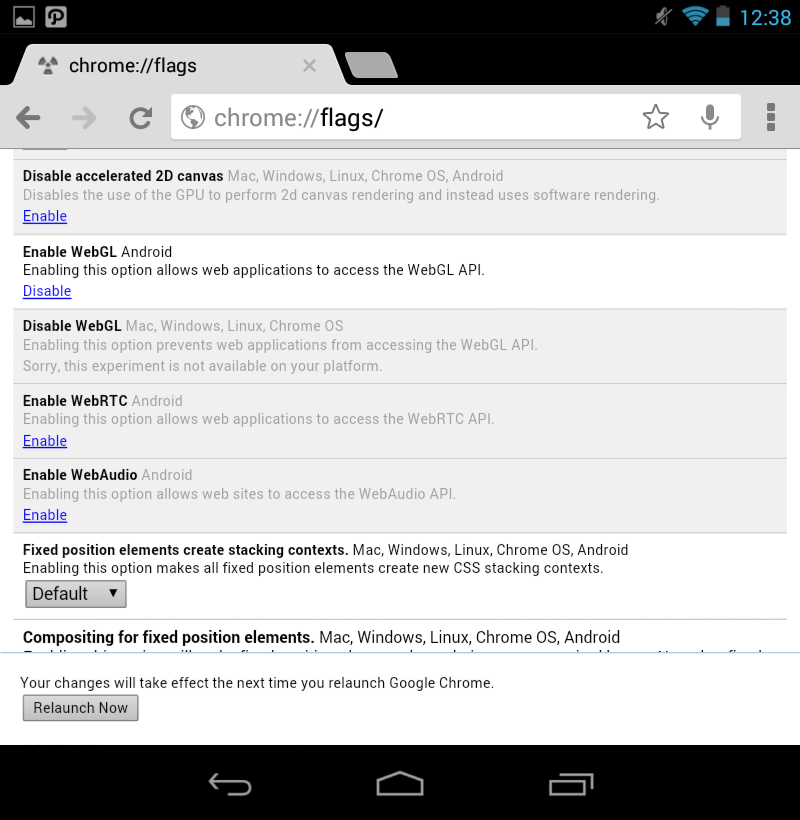
\includegraphics[width=10cm]{pic/min-chrome-flag.png}
\end{center}
\caption{Za delovanje WebGLa v brskalniku Chrome na Androidu je potrebno nastaviti posebno zastavico.}
\label{minchromeflag}
\end{figure} 

\begin{figure}
\begin{center}
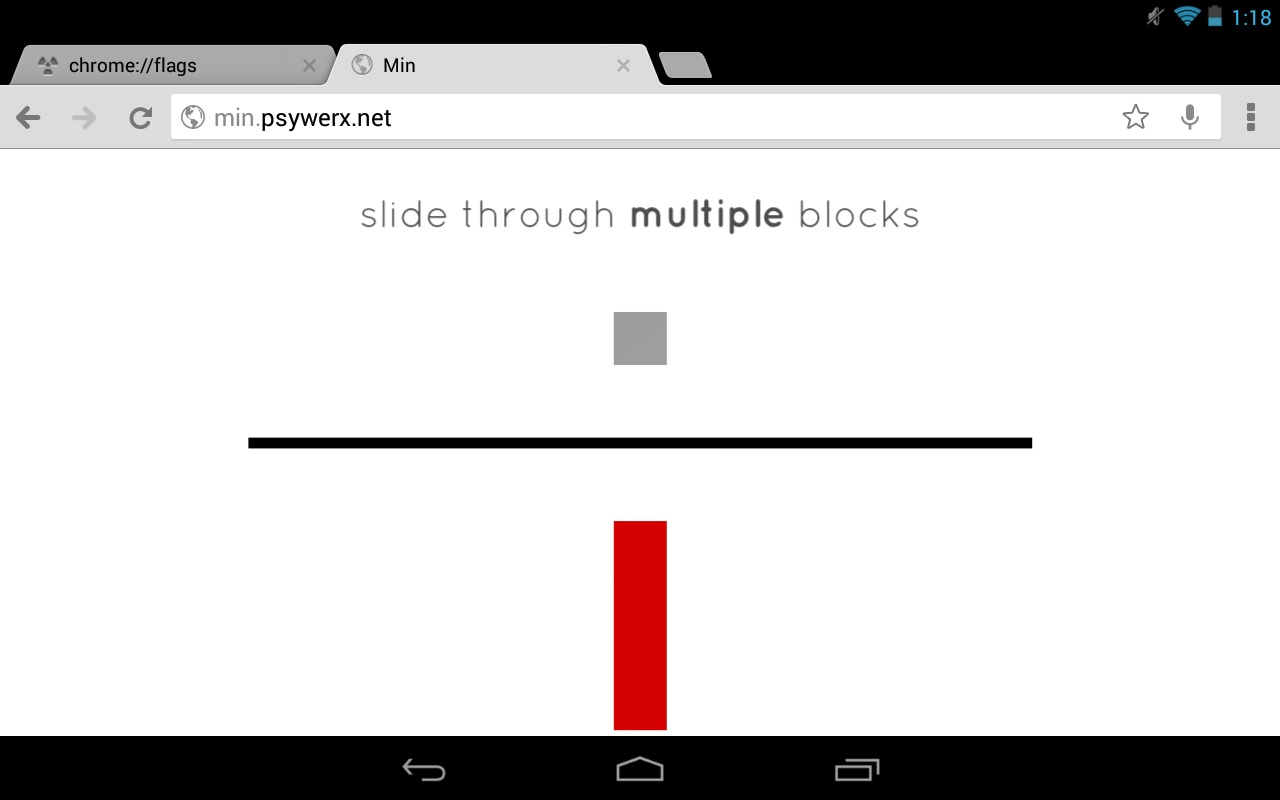
\includegraphics[width=12cm]{pic/min-chrome.png}
\end{center}
\caption{Delovanje igre v mobilnem brskalniku Chrome.}
\label{minchrome}
\end{figure}

\section{3D grafični prikaz aktivnost uporabnikov IRC kanala}

Naš zadnji primer je 3D grafični prikaz aktivnost uporabnikov IRC kanala glede na dan v tednu in uro v dnevu. Graf prikazuje podatke zajete v obdobju enega leta. Vsak dan ima 24 stolpcev za vsako uro v dnevu. Celoten graf vsebuje 7 vrst po 24 stolpcev, kar skupaj znaša 168 stolpcev. Višina posameznega stolpca ponazarja količino aktivnosti.

Aplikacija je sestavljena iz dveh delov. Prvi del je preprosta skripta napisana v programskem jeziku Python in je zadolžena za pripravo ustreznih podatkov. Linearno se sprehodili čez celoten zapisnik pogovorov in vsako aktivnost zabeležili v 2D polje. 2D polje je sestavljeno iz 168 številskih vrednosti, kjer vsaka vrednost predstavlja količino aktivnosti na določen dan v tednu ob določeni uri. To polje se izvozi v tekstovno datoteko.

Drugi del aplikacije uporabi pripravljene podatke v tekstovni datoteki za izris 3D grafa. Za izrisovanje smo uporabili programski jezik C++ in pogon Gameplay. Rezultat aplikacije je viden na sliki \ref{cppgraph}.

\subsection{Uporabljena metoda}

Glavni imenik Gameplay projekta vsebuje imenik \texttt{res}, ki vsebuje vsa sredstva, ki jih aplikacija potrebuje. Sem spadajo materiali uporabljeni v aplikaciji, izvorna koda uporabljenih GLSL programov, teksture in fonti. Pod sredstva lahko dodamo tudi izvoženo sceno iz grafičnih programov Maya ali Blender, vendar jih moramo pred uporabo pretvoriti v poseben binarni format. Orodje za pretvorbo je priloženo.

Imenik \texttt{src} vsebuje vso izvorno kodo programa, imenik \texttt{android} pa vse potrebno za grajenje projekta za platformo Android. V glavnem imeniku je tudi imenik \texttt{.xcodeproj}, ki vsebuje vse potrebno za grajenje za iOS.

\begin{figure}
\begin{center}
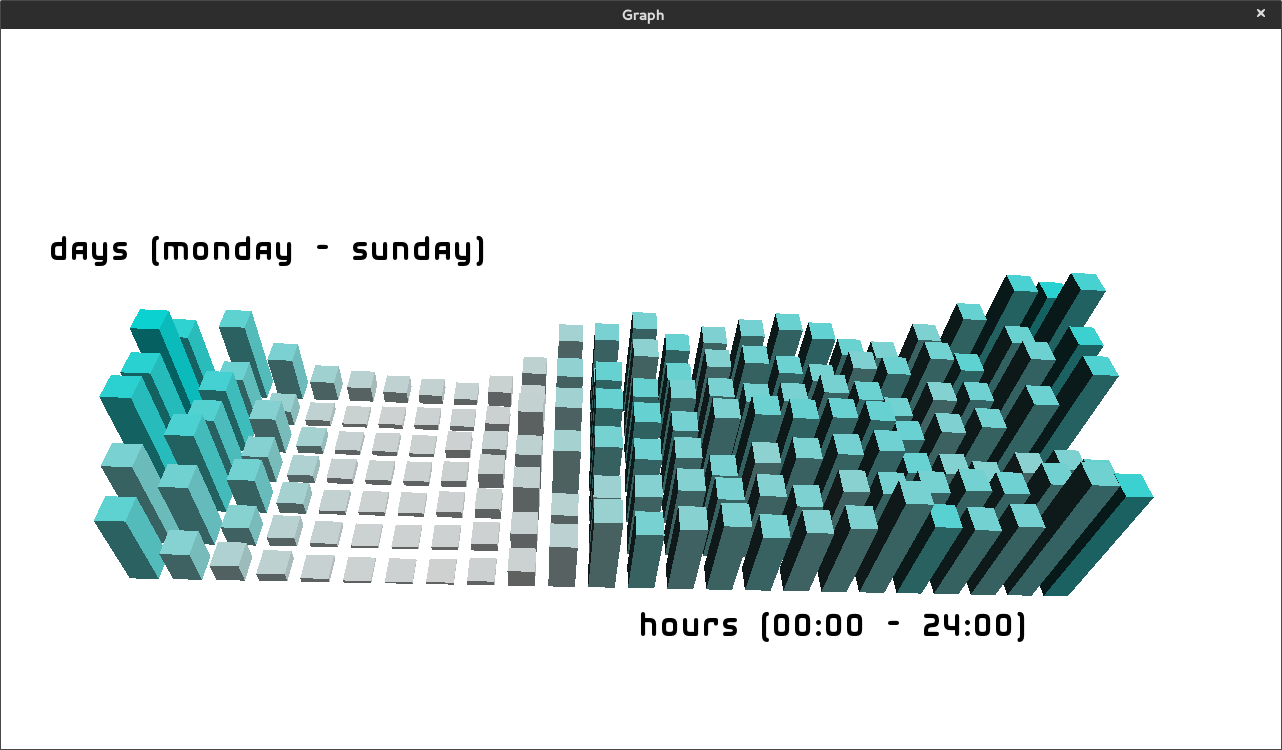
\includegraphics[width=12cm]{pic/cpp.png}
\end{center}
\caption{3D graf aktivnosti narejen z uporabo gameplay C++ knjižnice}
\label{cppgraph}
\end{figure}

Grajenje aplikacije poteka v dveh fazah. Najprej poženemo ukaz \texttt{cmake}, ki pripravi vse potrebne knjižnice, ki so potrebne za prevajanje aplikacije na izbrani platformi. Ko orodje \texttt{cmake} opravi svoje delo, imamo vse pripravljeno za prevajanje aplikacije z ukazom \texttt{make}, ki pripravi binarno datoteko, ki jo lahko zaženemo. Na ta način dobimo izvedljivo binarno datoteko za operacijski sistem Linux. Na operacijskem sistemu Windows se za grajenje aplikacije uporablja integrirano razvijalsko orodje Visual Studio. Ko Gameplay ustvari nov projekt, pripravi tudi konfiguracijsko datoteko za Visual Studio. Na podoben način se pripravi tudi datoteka za orodje Xcode, ki se uporablja za grajenje aplikacij na operacijskem sistemu Mac OSX. Znotraj projekta za Xcode so tudi navodila za grajenje iOS aplikacij. Za platformo Android se namesto ukaza \texttt{make} uporabi ukaz \texttt{ndk-build}, ki je del Android paketa za razvoj domorodnih aplikacij. \texttt{ndk-build} pripravi knjižnico, do katere lahko dostopamo tudi iz programskega jezika Java.  

\subsection{Prednosti izbora metode}

Gameplay pogon pripravi vse potrebno za razvoj medplatformnih aplikacij. Navodila za grajenje aplikacij na različnih platformah so preprosta in dobro dokumentirana.

\subsection{Slabosti izbora metode}

Dokumentacija za uporabo pogona je na določenih mestih pomanjkljiva, tako da je med razvojem potrebno pogledati v izvorno kodo pogona ali priloženih primerov. 



%Primer Min je bil narejen s pomočjo knjižnice LibGDX. Za svoje delovanje izrablja %zmoglivosti OpenGL ES 2.0. 


